% Created by tikzDevice version 0.12.3.1 on 2022-09-24 18:17:36
% !TEX encoding = UTF-8 Unicode
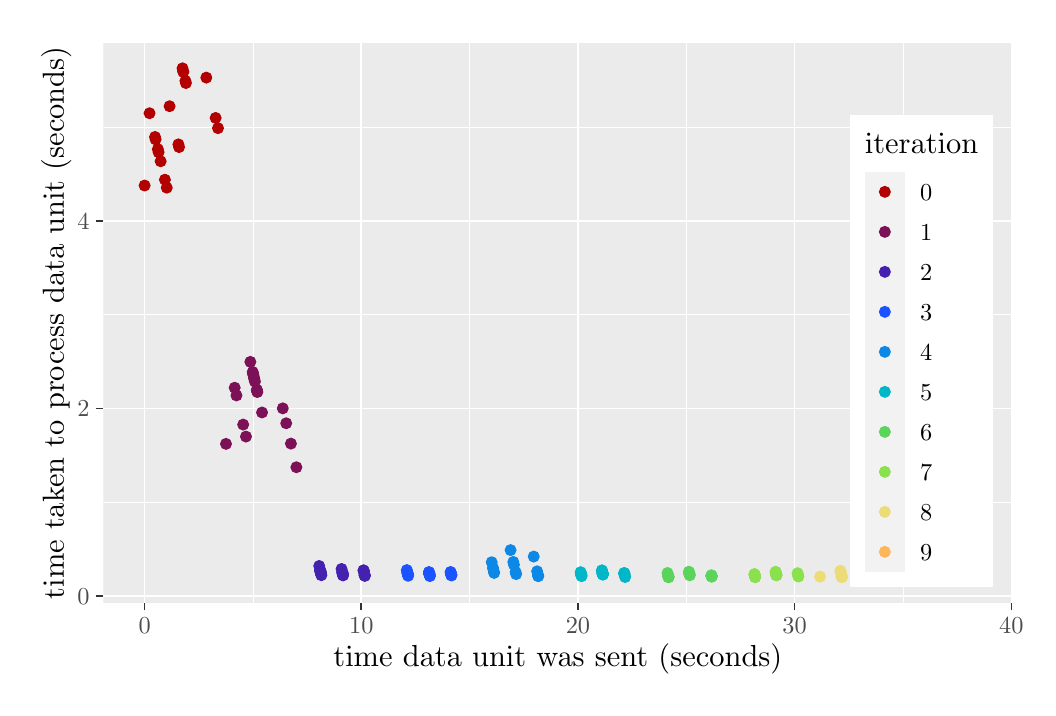
\begin{tikzpicture}[x=1pt,y=1pt]
\definecolor{fillColor}{RGB}{255,255,255}
\path[use as bounding box,fill=fillColor,fill opacity=0.00] (0,0) rectangle (361.35,238.49);
\begin{scope}
\path[clip] (  0.00,  0.00) rectangle (361.35,238.49);
\definecolor{drawColor}{RGB}{255,255,255}
\definecolor{fillColor}{RGB}{255,255,255}

\path[draw=drawColor,line width= 0.6pt,line join=round,line cap=round,fill=fillColor] (  0.00,  0.00) rectangle (361.35,238.49);
\end{scope}
\begin{scope}
\path[clip] ( 27.31, 30.69) rectangle (355.85,232.99);
\definecolor{fillColor}{gray}{0.92}

\path[fill=fillColor] ( 27.31, 30.69) rectangle (355.85,232.99);
\definecolor{drawColor}{RGB}{255,255,255}

\path[draw=drawColor,line width= 0.3pt,line join=round] ( 27.31, 66.98) --
	(355.85, 66.98);

\path[draw=drawColor,line width= 0.3pt,line join=round] ( 27.31,134.73) --
	(355.85,134.73);

\path[draw=drawColor,line width= 0.3pt,line join=round] ( 27.31,202.49) --
	(355.85,202.49);

\path[draw=drawColor,line width= 0.3pt,line join=round] ( 81.40, 30.69) --
	( 81.40,232.99);

\path[draw=drawColor,line width= 0.3pt,line join=round] (159.70, 30.69) --
	(159.70,232.99);

\path[draw=drawColor,line width= 0.3pt,line join=round] (238.00, 30.69) --
	(238.00,232.99);

\path[draw=drawColor,line width= 0.3pt,line join=round] (316.30, 30.69) --
	(316.30,232.99);

\path[draw=drawColor,line width= 0.6pt,line join=round] ( 27.31, 33.11) --
	(355.85, 33.11);

\path[draw=drawColor,line width= 0.6pt,line join=round] ( 27.31,100.86) --
	(355.85,100.86);

\path[draw=drawColor,line width= 0.6pt,line join=round] ( 27.31,168.61) --
	(355.85,168.61);

\path[draw=drawColor,line width= 0.6pt,line join=round] ( 42.25, 30.69) --
	( 42.25,232.99);

\path[draw=drawColor,line width= 0.6pt,line join=round] (120.55, 30.69) --
	(120.55,232.99);

\path[draw=drawColor,line width= 0.6pt,line join=round] (198.85, 30.69) --
	(198.85,232.99);

\path[draw=drawColor,line width= 0.6pt,line join=round] (277.15, 30.69) --
	(277.15,232.99);

\path[draw=drawColor,line width= 0.6pt,line join=round] (355.45, 30.69) --
	(355.45,232.99);
\definecolor{drawColor}{RGB}{179,0,0}
\definecolor{fillColor}{RGB}{179,0,0}

\path[draw=drawColor,line width= 0.4pt,line join=round,line cap=round,fill=fillColor] ( 42.25,181.45) circle (  1.96);

\path[draw=drawColor,line width= 0.4pt,line join=round,line cap=round,fill=fillColor] ( 44.04,207.57) circle (  1.96);

\path[draw=drawColor,line width= 0.4pt,line join=round,line cap=round,fill=fillColor] ( 46.22,198.12) circle (  1.96);

\path[draw=drawColor,line width= 0.4pt,line join=round,line cap=round,fill=fillColor] ( 46.02,199.00) circle (  1.96);

\path[draw=drawColor,line width= 0.4pt,line join=round,line cap=round,fill=fillColor] ( 50.26,180.67) circle (  1.96);

\path[draw=drawColor,line width= 0.4pt,line join=round,line cap=round,fill=fillColor] ( 49.59,183.55) circle (  1.96);
\definecolor{drawColor}{RGB}{124,17,88}
\definecolor{fillColor}{RGB}{124,17,88}

\path[draw=drawColor,line width= 0.4pt,line join=round,line cap=round,fill=fillColor] ( 71.66, 88.09) circle (  1.96);
\definecolor{drawColor}{RGB}{179,0,0}
\definecolor{fillColor}{RGB}{179,0,0}

\path[draw=drawColor,line width= 0.4pt,line join=round,line cap=round,fill=fillColor] ( 47.04,194.59) circle (  1.96);

\path[draw=drawColor,line width= 0.4pt,line join=round,line cap=round,fill=fillColor] ( 48.05,190.22) circle (  1.96);

\path[draw=drawColor,line width= 0.4pt,line join=round,line cap=round,fill=fillColor] ( 47.30,193.48) circle (  1.96);
\definecolor{drawColor}{RGB}{124,17,88}
\definecolor{fillColor}{RGB}{124,17,88}

\path[draw=drawColor,line width= 0.4pt,line join=round,line cap=round,fill=fillColor] ( 78.88, 90.73) circle (  1.96);
\definecolor{drawColor}{RGB}{179,0,0}
\definecolor{fillColor}{RGB}{179,0,0}

\path[draw=drawColor,line width= 0.4pt,line join=round,line cap=round,fill=fillColor] ( 54.47,196.32) circle (  1.96);
\definecolor{drawColor}{RGB}{124,17,88}
\definecolor{fillColor}{RGB}{124,17,88}

\path[draw=drawColor,line width= 0.4pt,line join=round,line cap=round,fill=fillColor] ( 77.87, 95.07) circle (  1.96);
\definecolor{drawColor}{RGB}{179,0,0}
\definecolor{fillColor}{RGB}{179,0,0}

\path[draw=drawColor,line width= 0.4pt,line join=round,line cap=round,fill=fillColor] ( 54.70,195.34) circle (  1.96);
\definecolor{drawColor}{RGB}{124,17,88}
\definecolor{fillColor}{RGB}{124,17,88}

\path[draw=drawColor,line width= 0.4pt,line join=round,line cap=round,fill=fillColor] ( 75.44,105.60) circle (  1.96);

\path[draw=drawColor,line width= 0.4pt,line join=round,line cap=round,fill=fillColor] ( 74.80,108.38) circle (  1.96);
\definecolor{drawColor}{RGB}{179,0,0}
\definecolor{fillColor}{RGB}{179,0,0}

\path[draw=drawColor,line width= 0.4pt,line join=round,line cap=round,fill=fillColor] ( 51.28,210.11) circle (  1.96);
\definecolor{drawColor}{RGB}{124,17,88}
\definecolor{fillColor}{RGB}{124,17,88}

\path[draw=drawColor,line width= 0.4pt,line join=round,line cap=round,fill=fillColor] ( 81.92,111.43) circle (  1.96);

\path[draw=drawColor,line width= 0.4pt,line join=round,line cap=round,fill=fillColor] ( 82.83,107.50) circle (  1.96);

\path[draw=drawColor,line width= 0.4pt,line join=round,line cap=round,fill=fillColor] ( 82.81,107.60) circle (  1.96);

\path[draw=drawColor,line width= 0.4pt,line join=round,line cap=round,fill=fillColor] ( 82.11,110.61) circle (  1.96);

\path[draw=drawColor,line width= 0.4pt,line join=round,line cap=round,fill=fillColor] ( 82.99,106.82) circle (  1.96);

\path[draw=drawColor,line width= 0.4pt,line join=round,line cap=round,fill=fillColor] ( 81.31,114.07) circle (  1.96);

\path[draw=drawColor,line width= 0.4pt,line join=round,line cap=round,fill=fillColor] ( 81.78,112.04) circle (  1.96);
\definecolor{drawColor}{RGB}{179,0,0}
\definecolor{fillColor}{RGB}{179,0,0}

\path[draw=drawColor,line width= 0.4pt,line join=round,line cap=round,fill=fillColor] ( 57.18,218.48) circle (  1.96);
\definecolor{drawColor}{RGB}{124,17,88}
\definecolor{fillColor}{RGB}{124,17,88}

\path[draw=drawColor,line width= 0.4pt,line join=round,line cap=round,fill=fillColor] ( 80.47,117.73) circle (  1.96);

\path[draw=drawColor,line width= 0.4pt,line join=round,line cap=round,fill=fillColor] ( 82.88,107.26) circle (  1.96);

\path[draw=drawColor,line width= 0.4pt,line join=round,line cap=round,fill=fillColor] ( 81.44,113.53) circle (  1.96);

\path[draw=drawColor,line width= 0.4pt,line join=round,line cap=round,fill=fillColor] ( 81.56,112.99) circle (  1.96);
\definecolor{drawColor}{RGB}{179,0,0}
\definecolor{fillColor}{RGB}{179,0,0}

\path[draw=drawColor,line width= 0.4pt,line join=round,line cap=round,fill=fillColor] ( 56.25,222.47) circle (  1.96);

\path[draw=drawColor,line width= 0.4pt,line join=round,line cap=round,fill=fillColor] ( 55.95,223.80) circle (  1.96);

\path[draw=drawColor,line width= 0.4pt,line join=round,line cap=round,fill=fillColor] ( 56.18,222.81) circle (  1.96);

\path[draw=drawColor,line width= 0.4pt,line join=round,line cap=round,fill=fillColor] ( 57.00,219.26) circle (  1.96);
\definecolor{drawColor}{RGB}{124,17,88}
\definecolor{fillColor}{RGB}{124,17,88}

\path[draw=drawColor,line width= 0.4pt,line join=round,line cap=round,fill=fillColor] ( 84.69, 99.44) circle (  1.96);

\path[draw=drawColor,line width= 0.4pt,line join=round,line cap=round,fill=fillColor] ( 92.18,100.93) circle (  1.96);
\definecolor{drawColor}{RGB}{179,0,0}
\definecolor{fillColor}{RGB}{179,0,0}

\path[draw=drawColor,line width= 0.4pt,line join=round,line cap=round,fill=fillColor] ( 64.55,220.44) circle (  1.96);

\path[draw=drawColor,line width= 0.4pt,line join=round,line cap=round,fill=fillColor] ( 67.92,205.87) circle (  1.96);
\definecolor{drawColor}{RGB}{124,17,88}
\definecolor{fillColor}{RGB}{124,17,88}

\path[draw=drawColor,line width= 0.4pt,line join=round,line cap=round,fill=fillColor] ( 93.42, 95.54) circle (  1.96);
\definecolor{drawColor}{RGB}{179,0,0}
\definecolor{fillColor}{RGB}{179,0,0}

\path[draw=drawColor,line width= 0.4pt,line join=round,line cap=round,fill=fillColor] ( 68.77,202.18) circle (  1.96);
\definecolor{drawColor}{RGB}{124,17,88}
\definecolor{fillColor}{RGB}{124,17,88}

\path[draw=drawColor,line width= 0.4pt,line join=round,line cap=round,fill=fillColor] ( 95.12, 88.19) circle (  1.96);

\path[draw=drawColor,line width= 0.4pt,line join=round,line cap=round,fill=fillColor] ( 97.10, 79.65) circle (  1.96);
\definecolor{drawColor}{RGB}{68,33,175}
\definecolor{fillColor}{RGB}{68,33,175}

\path[draw=drawColor,line width= 0.4pt,line join=round,line cap=round,fill=fillColor] (105.83, 41.88) circle (  1.96);

\path[draw=drawColor,line width= 0.4pt,line join=round,line cap=round,fill=fillColor] (105.98, 41.20) circle (  1.96);

\path[draw=drawColor,line width= 0.4pt,line join=round,line cap=round,fill=fillColor] (106.12, 40.63) circle (  1.96);

\path[draw=drawColor,line width= 0.4pt,line join=round,line cap=round,fill=fillColor] (105.85, 41.78) circle (  1.96);

\path[draw=drawColor,line width= 0.4pt,line join=round,line cap=round,fill=fillColor] (105.69, 42.49) circle (  1.96);

\path[draw=drawColor,line width= 0.4pt,line join=round,line cap=round,fill=fillColor] (105.34, 43.98) circle (  1.96);

\path[draw=drawColor,line width= 0.4pt,line join=round,line cap=round,fill=fillColor] (105.70, 42.42) circle (  1.96);

\path[draw=drawColor,line width= 0.4pt,line join=round,line cap=round,fill=fillColor] (105.98, 41.24) circle (  1.96);

\path[draw=drawColor,line width= 0.4pt,line join=round,line cap=round,fill=fillColor] (105.94, 41.37) circle (  1.96);

\path[draw=drawColor,line width= 0.4pt,line join=round,line cap=round,fill=fillColor] (105.76, 42.15) circle (  1.96);

\path[draw=drawColor,line width= 0.4pt,line join=round,line cap=round,fill=fillColor] (113.87, 40.97) circle (  1.96);

\path[draw=drawColor,line width= 0.4pt,line join=round,line cap=round,fill=fillColor] (113.74, 41.51) circle (  1.96);

\path[draw=drawColor,line width= 0.4pt,line join=round,line cap=round,fill=fillColor] (113.42, 42.90) circle (  1.96);

\path[draw=drawColor,line width= 0.4pt,line join=round,line cap=round,fill=fillColor] (113.71, 41.64) circle (  1.96);

\path[draw=drawColor,line width= 0.4pt,line join=round,line cap=round,fill=fillColor] (113.70, 41.71) circle (  1.96);

\path[draw=drawColor,line width= 0.4pt,line join=round,line cap=round,fill=fillColor] (113.95, 40.63) circle (  1.96);

\path[draw=drawColor,line width= 0.4pt,line join=round,line cap=round,fill=fillColor] (113.86, 41.00) circle (  1.96);

\path[draw=drawColor,line width= 0.4pt,line join=round,line cap=round,fill=fillColor] (113.95, 40.59) circle (  1.96);

\path[draw=drawColor,line width= 0.4pt,line join=round,line cap=round,fill=fillColor] (121.37, 42.39) circle (  1.96);

\path[draw=drawColor,line width= 0.4pt,line join=round,line cap=round,fill=fillColor] (121.49, 41.85) circle (  1.96);

\path[draw=drawColor,line width= 0.4pt,line join=round,line cap=round,fill=fillColor] (121.38, 42.35) circle (  1.96);

\path[draw=drawColor,line width= 0.4pt,line join=round,line cap=round,fill=fillColor] (121.80, 40.53) circle (  1.96);

\path[draw=drawColor,line width= 0.4pt,line join=round,line cap=round,fill=fillColor] (121.77, 40.66) circle (  1.96);

\path[draw=drawColor,line width= 0.4pt,line join=round,line cap=round,fill=fillColor] (121.42, 42.19) circle (  1.96);

\path[draw=drawColor,line width= 0.4pt,line join=round,line cap=round,fill=fillColor] (121.75, 40.76) circle (  1.96);

\path[draw=drawColor,line width= 0.4pt,line join=round,line cap=round,fill=fillColor] (121.83, 40.39) circle (  1.96);
\definecolor{drawColor}{RGB}{26,83,255}
\definecolor{fillColor}{RGB}{26,83,255}

\path[draw=drawColor,line width= 0.4pt,line join=round,line cap=round,fill=fillColor] (137.42, 40.69) circle (  1.96);

\path[draw=drawColor,line width= 0.4pt,line join=round,line cap=round,fill=fillColor] (137.48, 40.42) circle (  1.96);

\path[draw=drawColor,line width= 0.4pt,line join=round,line cap=round,fill=fillColor] (137.26, 41.41) circle (  1.96);

\path[draw=drawColor,line width= 0.4pt,line join=round,line cap=round,fill=fillColor] (137.01, 42.49) circle (  1.96);

\path[draw=drawColor,line width= 0.4pt,line join=round,line cap=round,fill=fillColor] (137.30, 41.24) circle (  1.96);

\path[draw=drawColor,line width= 0.4pt,line join=round,line cap=round,fill=fillColor] (137.14, 41.91) circle (  1.96);

\path[draw=drawColor,line width= 0.4pt,line join=round,line cap=round,fill=fillColor] (137.30, 41.20) circle (  1.96);

\path[draw=drawColor,line width= 0.4pt,line join=round,line cap=round,fill=fillColor] (137.41, 40.73) circle (  1.96);

\path[draw=drawColor,line width= 0.4pt,line join=round,line cap=round,fill=fillColor] (145.22, 40.83) circle (  1.96);

\path[draw=drawColor,line width= 0.4pt,line join=round,line cap=round,fill=fillColor] (145.11, 41.30) circle (  1.96);

\path[draw=drawColor,line width= 0.4pt,line join=round,line cap=round,fill=fillColor] (145.06, 41.54) circle (  1.96);

\path[draw=drawColor,line width= 0.4pt,line join=round,line cap=round,fill=fillColor] (145.34, 40.32) circle (  1.96);

\path[draw=drawColor,line width= 0.4pt,line join=round,line cap=round,fill=fillColor] (145.16, 41.10) circle (  1.96);

\path[draw=drawColor,line width= 0.4pt,line join=round,line cap=round,fill=fillColor] (145.08, 41.44) circle (  1.96);

\path[draw=drawColor,line width= 0.4pt,line join=round,line cap=round,fill=fillColor] (145.28, 40.56) circle (  1.96);

\path[draw=drawColor,line width= 0.4pt,line join=round,line cap=round,fill=fillColor] (145.00, 41.78) circle (  1.96);

\path[draw=drawColor,line width= 0.4pt,line join=round,line cap=round,fill=fillColor] (145.17, 41.03) circle (  1.96);

\path[draw=drawColor,line width= 0.4pt,line join=round,line cap=round,fill=fillColor] (145.03, 41.64) circle (  1.96);

\path[draw=drawColor,line width= 0.4pt,line join=round,line cap=round,fill=fillColor] (145.13, 41.20) circle (  1.96);

\path[draw=drawColor,line width= 0.4pt,line join=round,line cap=round,fill=fillColor] (153.04, 40.86) circle (  1.96);

\path[draw=drawColor,line width= 0.4pt,line join=round,line cap=round,fill=fillColor] (152.92, 41.37) circle (  1.96);

\path[draw=drawColor,line width= 0.4pt,line join=round,line cap=round,fill=fillColor] (152.91, 41.44) circle (  1.96);

\path[draw=drawColor,line width= 0.4pt,line join=round,line cap=round,fill=fillColor] (152.82, 41.81) circle (  1.96);

\path[draw=drawColor,line width= 0.4pt,line join=round,line cap=round,fill=fillColor] (153.03, 40.93) circle (  1.96);

\path[draw=drawColor,line width= 0.4pt,line join=round,line cap=round,fill=fillColor] (153.12, 40.53) circle (  1.96);

\path[draw=drawColor,line width= 0.4pt,line join=round,line cap=round,fill=fillColor] (153.06, 40.80) circle (  1.96);
\definecolor{drawColor}{RGB}{13,136,230}
\definecolor{fillColor}{RGB}{13,136,230}

\path[draw=drawColor,line width= 0.4pt,line join=round,line cap=round,fill=fillColor] (168.14, 43.30) circle (  1.96);

\path[draw=drawColor,line width= 0.4pt,line join=round,line cap=round,fill=fillColor] (168.48, 41.85) circle (  1.96);

\path[draw=drawColor,line width= 0.4pt,line join=round,line cap=round,fill=fillColor] (168.22, 42.93) circle (  1.96);

\path[draw=drawColor,line width= 0.4pt,line join=round,line cap=round,fill=fillColor] (168.56, 41.47) circle (  1.96);

\path[draw=drawColor,line width= 0.4pt,line join=round,line cap=round,fill=fillColor] (167.67, 45.34) circle (  1.96);

\path[draw=drawColor,line width= 0.4pt,line join=round,line cap=round,fill=fillColor] (175.48, 45.44) circle (  1.96);

\path[draw=drawColor,line width= 0.4pt,line join=round,line cap=round,fill=fillColor] (174.49, 49.71) circle (  1.96);

\path[draw=drawColor,line width= 0.4pt,line join=round,line cap=round,fill=fillColor] (176.49, 41.03) circle (  1.96);

\path[draw=drawColor,line width= 0.4pt,line join=round,line cap=round,fill=fillColor] (175.71, 44.42) circle (  1.96);

\path[draw=drawColor,line width= 0.4pt,line join=round,line cap=round,fill=fillColor] (176.31, 41.81) circle (  1.96);

\path[draw=drawColor,line width= 0.4pt,line join=round,line cap=round,fill=fillColor] (184.09, 42.05) circle (  1.96);

\path[draw=drawColor,line width= 0.4pt,line join=round,line cap=round,fill=fillColor] (182.86, 47.37) circle (  1.96);

\path[draw=drawColor,line width= 0.4pt,line join=round,line cap=round,fill=fillColor] (184.50, 40.29) circle (  1.96);

\path[draw=drawColor,line width= 0.4pt,line join=round,line cap=round,fill=fillColor] (184.37, 40.83) circle (  1.96);

\path[draw=drawColor,line width= 0.4pt,line join=round,line cap=round,fill=fillColor] (184.48, 40.36) circle (  1.96);
\definecolor{drawColor}{RGB}{0,183,199}
\definecolor{fillColor}{RGB}{0,183,199}

\path[draw=drawColor,line width= 0.4pt,line join=round,line cap=round,fill=fillColor] (200.16, 40.29) circle (  1.96);

\path[draw=drawColor,line width= 0.4pt,line join=round,line cap=round,fill=fillColor] (200.01, 40.93) circle (  1.96);

\path[draw=drawColor,line width= 0.4pt,line join=round,line cap=round,fill=fillColor] (200.05, 40.73) circle (  1.96);

\path[draw=drawColor,line width= 0.4pt,line join=round,line cap=round,fill=fillColor] (200.01, 40.90) circle (  1.96);

\path[draw=drawColor,line width= 0.4pt,line join=round,line cap=round,fill=fillColor] (199.82, 41.74) circle (  1.96);

\path[draw=drawColor,line width= 0.4pt,line join=round,line cap=round,fill=fillColor] (199.93, 41.27) circle (  1.96);

\path[draw=drawColor,line width= 0.4pt,line join=round,line cap=round,fill=fillColor] (200.06, 40.69) circle (  1.96);

\path[draw=drawColor,line width= 0.4pt,line join=round,line cap=round,fill=fillColor] (207.77, 41.24) circle (  1.96);

\path[draw=drawColor,line width= 0.4pt,line join=round,line cap=round,fill=fillColor] (207.85, 40.86) circle (  1.96);

\path[draw=drawColor,line width= 0.4pt,line join=round,line cap=round,fill=fillColor] (207.76, 41.27) circle (  1.96);

\path[draw=drawColor,line width= 0.4pt,line join=round,line cap=round,fill=fillColor] (207.52, 42.29) circle (  1.96);

\path[draw=drawColor,line width= 0.4pt,line join=round,line cap=round,fill=fillColor] (207.70, 41.54) circle (  1.96);

\path[draw=drawColor,line width= 0.4pt,line join=round,line cap=round,fill=fillColor] (207.70, 41.51) circle (  1.96);

\path[draw=drawColor,line width= 0.4pt,line join=round,line cap=round,fill=fillColor] (207.84, 40.90) circle (  1.96);

\path[draw=drawColor,line width= 0.4pt,line join=round,line cap=round,fill=fillColor] (207.75, 41.30) circle (  1.96);

\path[draw=drawColor,line width= 0.4pt,line join=round,line cap=round,fill=fillColor] (207.50, 42.39) circle (  1.96);

\path[draw=drawColor,line width= 0.4pt,line join=round,line cap=round,fill=fillColor] (207.74, 41.34) circle (  1.96);

\path[draw=drawColor,line width= 0.4pt,line join=round,line cap=round,fill=fillColor] (207.79, 41.13) circle (  1.96);

\path[draw=drawColor,line width= 0.4pt,line join=round,line cap=round,fill=fillColor] (207.81, 41.07) circle (  1.96);

\path[draw=drawColor,line width= 0.4pt,line join=round,line cap=round,fill=fillColor] (215.60, 41.24) circle (  1.96);

\path[draw=drawColor,line width= 0.4pt,line join=round,line cap=round,fill=fillColor] (215.89, 39.98) circle (  1.96);

\path[draw=drawColor,line width= 0.4pt,line join=round,line cap=round,fill=fillColor] (215.75, 40.59) circle (  1.96);

\path[draw=drawColor,line width= 0.4pt,line join=round,line cap=round,fill=fillColor] (215.55, 41.44) circle (  1.96);

\path[draw=drawColor,line width= 0.4pt,line join=round,line cap=round,fill=fillColor] (215.67, 40.90) circle (  1.96);

\path[draw=drawColor,line width= 0.4pt,line join=round,line cap=round,fill=fillColor] (215.59, 41.27) circle (  1.96);

\path[draw=drawColor,line width= 0.4pt,line join=round,line cap=round,fill=fillColor] (215.57, 41.34) circle (  1.96);
\definecolor{drawColor}{RGB}{90,212,90}
\definecolor{fillColor}{RGB}{90,212,90}

\path[draw=drawColor,line width= 0.4pt,line join=round,line cap=round,fill=fillColor] (231.54, 40.02) circle (  1.96);

\path[draw=drawColor,line width= 0.4pt,line join=round,line cap=round,fill=fillColor] (231.53, 40.05) circle (  1.96);

\path[draw=drawColor,line width= 0.4pt,line join=round,line cap=round,fill=fillColor] (231.42, 40.53) circle (  1.96);

\path[draw=drawColor,line width= 0.4pt,line join=round,line cap=round,fill=fillColor] (231.57, 39.88) circle (  1.96);

\path[draw=drawColor,line width= 0.4pt,line join=round,line cap=round,fill=fillColor] (231.46, 40.36) circle (  1.96);

\path[draw=drawColor,line width= 0.4pt,line join=round,line cap=round,fill=fillColor] (231.55, 39.98) circle (  1.96);

\path[draw=drawColor,line width= 0.4pt,line join=round,line cap=round,fill=fillColor] (231.36, 40.80) circle (  1.96);

\path[draw=drawColor,line width= 0.4pt,line join=round,line cap=round,fill=fillColor] (231.21, 41.44) circle (  1.96);

\path[draw=drawColor,line width= 0.4pt,line join=round,line cap=round,fill=fillColor] (238.93, 41.91) circle (  1.96);

\path[draw=drawColor,line width= 0.4pt,line join=round,line cap=round,fill=fillColor] (239.00, 41.61) circle (  1.96);

\path[draw=drawColor,line width= 0.4pt,line join=round,line cap=round,fill=fillColor] (239.12, 41.10) circle (  1.96);

\path[draw=drawColor,line width= 0.4pt,line join=round,line cap=round,fill=fillColor] (239.18, 40.83) circle (  1.96);

\path[draw=drawColor,line width= 0.4pt,line join=round,line cap=round,fill=fillColor] (239.02, 41.51) circle (  1.96);

\path[draw=drawColor,line width= 0.4pt,line join=round,line cap=round,fill=fillColor] (239.24, 40.59) circle (  1.96);

\path[draw=drawColor,line width= 0.4pt,line join=round,line cap=round,fill=fillColor] (247.10, 40.42) circle (  1.96);

\path[draw=drawColor,line width= 0.4pt,line join=round,line cap=round,fill=fillColor] (247.14, 40.25) circle (  1.96);

\path[draw=drawColor,line width= 0.4pt,line join=round,line cap=round,fill=fillColor] (247.12, 40.36) circle (  1.96);

\path[draw=drawColor,line width= 0.4pt,line join=round,line cap=round,fill=fillColor] (247.06, 40.63) circle (  1.96);

\path[draw=drawColor,line width= 0.4pt,line join=round,line cap=round,fill=fillColor] (247.18, 40.08) circle (  1.96);

\path[draw=drawColor,line width= 0.4pt,line join=round,line cap=round,fill=fillColor] (247.14, 40.29) circle (  1.96);
\definecolor{drawColor}{RGB}{139,224,78}
\definecolor{fillColor}{RGB}{139,224,78}

\path[draw=drawColor,line width= 0.4pt,line join=round,line cap=round,fill=fillColor] (262.87, 39.95) circle (  1.96);

\path[draw=drawColor,line width= 0.4pt,line join=round,line cap=round,fill=fillColor] (262.67, 40.83) circle (  1.96);

\path[draw=drawColor,line width= 0.4pt,line join=round,line cap=round,fill=fillColor] (262.80, 40.25) circle (  1.96);

\path[draw=drawColor,line width= 0.4pt,line join=round,line cap=round,fill=fillColor] (262.62, 41.03) circle (  1.96);

\path[draw=drawColor,line width= 0.4pt,line join=round,line cap=round,fill=fillColor] (262.88, 39.92) circle (  1.96);

\path[draw=drawColor,line width= 0.4pt,line join=round,line cap=round,fill=fillColor] (262.74, 40.53) circle (  1.96);

\path[draw=drawColor,line width= 0.4pt,line join=round,line cap=round,fill=fillColor] (262.64, 40.97) circle (  1.96);

\path[draw=drawColor,line width= 0.4pt,line join=round,line cap=round,fill=fillColor] (262.76, 40.46) circle (  1.96);

\path[draw=drawColor,line width= 0.4pt,line join=round,line cap=round,fill=fillColor] (270.54, 40.66) circle (  1.96);

\path[draw=drawColor,line width= 0.4pt,line join=round,line cap=round,fill=fillColor] (270.56, 40.59) circle (  1.96);

\path[draw=drawColor,line width= 0.4pt,line join=round,line cap=round,fill=fillColor] (270.39, 41.30) circle (  1.96);

\path[draw=drawColor,line width= 0.4pt,line join=round,line cap=round,fill=fillColor] (270.45, 41.07) circle (  1.96);

\path[draw=drawColor,line width= 0.4pt,line join=round,line cap=round,fill=fillColor] (270.49, 40.86) circle (  1.96);

\path[draw=drawColor,line width= 0.4pt,line join=round,line cap=round,fill=fillColor] (270.44, 41.10) circle (  1.96);

\path[draw=drawColor,line width= 0.4pt,line join=round,line cap=round,fill=fillColor] (270.29, 41.74) circle (  1.96);

\path[draw=drawColor,line width= 0.4pt,line join=round,line cap=round,fill=fillColor] (270.52, 40.73) circle (  1.96);

\path[draw=drawColor,line width= 0.4pt,line join=round,line cap=round,fill=fillColor] (270.27, 41.85) circle (  1.96);

\path[draw=drawColor,line width= 0.4pt,line join=round,line cap=round,fill=fillColor] (270.37, 41.41) circle (  1.96);

\path[draw=drawColor,line width= 0.4pt,line join=round,line cap=round,fill=fillColor] (270.47, 40.97) circle (  1.96);

\path[draw=drawColor,line width= 0.4pt,line join=round,line cap=round,fill=fillColor] (278.21, 41.37) circle (  1.96);

\path[draw=drawColor,line width= 0.4pt,line join=round,line cap=round,fill=fillColor] (278.49, 40.15) circle (  1.96);

\path[draw=drawColor,line width= 0.4pt,line join=round,line cap=round,fill=fillColor] (278.38, 40.63) circle (  1.96);
\definecolor{drawColor}{RGB}{235,220,120}
\definecolor{fillColor}{RGB}{235,220,120}

\path[draw=drawColor,line width= 0.4pt,line join=round,line cap=round,fill=fillColor] (286.33, 40.12) circle (  1.96);

\path[draw=drawColor,line width= 0.4pt,line join=round,line cap=round,fill=fillColor] (294.14, 40.19) circle (  1.96);

\path[draw=drawColor,line width= 0.4pt,line join=round,line cap=round,fill=fillColor] (294.20, 39.92) circle (  1.96);

\path[draw=drawColor,line width= 0.4pt,line join=round,line cap=round,fill=fillColor] (294.19, 39.95) circle (  1.96);

\path[draw=drawColor,line width= 0.4pt,line join=round,line cap=round,fill=fillColor] (294.18, 40.02) circle (  1.96);

\path[draw=drawColor,line width= 0.4pt,line join=round,line cap=round,fill=fillColor] (293.67, 42.22) circle (  1.96);

\path[draw=drawColor,line width= 0.4pt,line join=round,line cap=round,fill=fillColor] (293.84, 41.47) circle (  1.96);

\path[draw=drawColor,line width= 0.4pt,line join=round,line cap=round,fill=fillColor] (294.11, 40.32) circle (  1.96);

\path[draw=drawColor,line width= 0.4pt,line join=round,line cap=round,fill=fillColor] (301.73, 41.20) circle (  1.96);

\path[draw=drawColor,line width= 0.4pt,line join=round,line cap=round,fill=fillColor] (301.70, 41.37) circle (  1.96);

\path[draw=drawColor,line width= 0.4pt,line join=round,line cap=round,fill=fillColor] (301.55, 42.02) circle (  1.96);

\path[draw=drawColor,line width= 0.4pt,line join=round,line cap=round,fill=fillColor] (301.94, 40.32) circle (  1.96);

\path[draw=drawColor,line width= 0.4pt,line join=round,line cap=round,fill=fillColor] (301.91, 40.46) circle (  1.96);

\path[draw=drawColor,line width= 0.4pt,line join=round,line cap=round,fill=fillColor] (301.79, 40.97) circle (  1.96);

\path[draw=drawColor,line width= 0.4pt,line join=round,line cap=round,fill=fillColor] (301.89, 40.53) circle (  1.96);

\path[draw=drawColor,line width= 0.4pt,line join=round,line cap=round,fill=fillColor] (301.65, 41.58) circle (  1.96);

\path[draw=drawColor,line width= 0.4pt,line join=round,line cap=round,fill=fillColor] (309.73, 40.49) circle (  1.96);

\path[draw=drawColor,line width= 0.4pt,line join=round,line cap=round,fill=fillColor] (309.68, 40.69) circle (  1.96);

\path[draw=drawColor,line width= 0.4pt,line join=round,line cap=round,fill=fillColor] (309.71, 40.59) circle (  1.96);
\definecolor{drawColor}{RGB}{255,181,90}
\definecolor{fillColor}{RGB}{255,181,90}

\path[draw=drawColor,line width= 0.4pt,line join=round,line cap=round,fill=fillColor] (317.59, 40.36) circle (  1.96);

\path[draw=drawColor,line width= 0.4pt,line join=round,line cap=round,fill=fillColor] (317.54, 40.59) circle (  1.96);

\path[draw=drawColor,line width= 0.4pt,line join=round,line cap=round,fill=fillColor] (325.41, 40.42) circle (  1.96);

\path[draw=drawColor,line width= 0.4pt,line join=round,line cap=round,fill=fillColor] (325.50, 40.02) circle (  1.96);

\path[draw=drawColor,line width= 0.4pt,line join=round,line cap=round,fill=fillColor] (325.30, 40.90) circle (  1.96);

\path[draw=drawColor,line width= 0.4pt,line join=round,line cap=round,fill=fillColor] (325.17, 41.44) circle (  1.96);

\path[draw=drawColor,line width= 0.4pt,line join=round,line cap=round,fill=fillColor] (325.33, 40.76) circle (  1.96);

\path[draw=drawColor,line width= 0.4pt,line join=round,line cap=round,fill=fillColor] (333.33, 40.02) circle (  1.96);

\path[draw=drawColor,line width= 0.4pt,line join=round,line cap=round,fill=fillColor] (333.27, 40.29) circle (  1.96);

\path[draw=drawColor,line width= 0.4pt,line join=round,line cap=round,fill=fillColor] (333.01, 41.41) circle (  1.96);

\path[draw=drawColor,line width= 0.4pt,line join=round,line cap=round,fill=fillColor] (333.06, 41.20) circle (  1.96);

\path[draw=drawColor,line width= 0.4pt,line join=round,line cap=round,fill=fillColor] (333.10, 41.00) circle (  1.96);

\path[draw=drawColor,line width= 0.4pt,line join=round,line cap=round,fill=fillColor] (333.09, 41.03) circle (  1.96);

\path[draw=drawColor,line width= 0.4pt,line join=round,line cap=round,fill=fillColor] (332.84, 42.15) circle (  1.96);

\path[draw=drawColor,line width= 0.4pt,line join=round,line cap=round,fill=fillColor] (332.82, 42.22) circle (  1.96);

\path[draw=drawColor,line width= 0.4pt,line join=round,line cap=round,fill=fillColor] (340.59, 42.49) circle (  1.96);

\path[draw=drawColor,line width= 0.4pt,line join=round,line cap=round,fill=fillColor] (340.92, 41.07) circle (  1.96);
\end{scope}
\begin{scope}
\path[clip] (  0.00,  0.00) rectangle (361.35,238.49);
\definecolor{drawColor}{gray}{0.30}

\node[text=drawColor,anchor=base east,inner sep=0pt, outer sep=0pt, scale=  0.88] at ( 22.36, 30.08) {0};

\node[text=drawColor,anchor=base east,inner sep=0pt, outer sep=0pt, scale=  0.88] at ( 22.36, 97.83) {2};

\node[text=drawColor,anchor=base east,inner sep=0pt, outer sep=0pt, scale=  0.88] at ( 22.36,165.58) {4};
\end{scope}
\begin{scope}
\path[clip] (  0.00,  0.00) rectangle (361.35,238.49);
\definecolor{drawColor}{gray}{0.20}

\path[draw=drawColor,line width= 0.6pt,line join=round] ( 24.56, 33.11) --
	( 27.31, 33.11);

\path[draw=drawColor,line width= 0.6pt,line join=round] ( 24.56,100.86) --
	( 27.31,100.86);

\path[draw=drawColor,line width= 0.6pt,line join=round] ( 24.56,168.61) --
	( 27.31,168.61);
\end{scope}
\begin{scope}
\path[clip] (  0.00,  0.00) rectangle (361.35,238.49);
\definecolor{drawColor}{gray}{0.20}

\path[draw=drawColor,line width= 0.6pt,line join=round] ( 42.25, 27.94) --
	( 42.25, 30.69);

\path[draw=drawColor,line width= 0.6pt,line join=round] (120.55, 27.94) --
	(120.55, 30.69);

\path[draw=drawColor,line width= 0.6pt,line join=round] (198.85, 27.94) --
	(198.85, 30.69);

\path[draw=drawColor,line width= 0.6pt,line join=round] (277.15, 27.94) --
	(277.15, 30.69);

\path[draw=drawColor,line width= 0.6pt,line join=round] (355.45, 27.94) --
	(355.45, 30.69);
\end{scope}
\begin{scope}
\path[clip] (  0.00,  0.00) rectangle (361.35,238.49);
\definecolor{drawColor}{gray}{0.30}

\node[text=drawColor,anchor=base,inner sep=0pt, outer sep=0pt, scale=  0.88] at ( 42.25, 19.68) {0};

\node[text=drawColor,anchor=base,inner sep=0pt, outer sep=0pt, scale=  0.88] at (120.55, 19.68) {10};

\node[text=drawColor,anchor=base,inner sep=0pt, outer sep=0pt, scale=  0.88] at (198.85, 19.68) {20};

\node[text=drawColor,anchor=base,inner sep=0pt, outer sep=0pt, scale=  0.88] at (277.15, 19.68) {30};

\node[text=drawColor,anchor=base,inner sep=0pt, outer sep=0pt, scale=  0.88] at (355.45, 19.68) {40};
\end{scope}
\begin{scope}
\path[clip] (  0.00,  0.00) rectangle (361.35,238.49);
\definecolor{drawColor}{RGB}{0,0,0}

\node[text=drawColor,anchor=base,inner sep=0pt, outer sep=0pt, scale=  1.10] at (191.58,  7.64) {time data unit was sent (seconds)};
\end{scope}
\begin{scope}
\path[clip] (  0.00,  0.00) rectangle (361.35,238.49);
\definecolor{drawColor}{RGB}{0,0,0}

\node[text=drawColor,rotate= 90.00,anchor=base,inner sep=0pt, outer sep=0pt, scale=  1.10] at ( 13.08,131.84) {time taken to process data unit (seconds)};
\end{scope}
\begin{scope}
\path[clip] (  0.00,  0.00) rectangle (361.35,238.49);
\definecolor{fillColor}{RGB}{255,255,255}

\path[fill=fillColor] (297.01, 36.35) rectangle (348.98,207.10);
\end{scope}
\begin{scope}
\path[clip] (  0.00,  0.00) rectangle (361.35,238.49);
\definecolor{drawColor}{RGB}{0,0,0}

\node[text=drawColor,anchor=base west,inner sep=0pt, outer sep=0pt, scale=  1.10] at (302.51,192.96) {iteration};
\end{scope}
\begin{scope}
\path[clip] (  0.00,  0.00) rectangle (361.35,238.49);
\definecolor{fillColor}{gray}{0.95}

\path[fill=fillColor] (302.51,171.93) rectangle (316.97,186.39);
\end{scope}
\begin{scope}
\path[clip] (  0.00,  0.00) rectangle (361.35,238.49);
\definecolor{drawColor}{RGB}{179,0,0}
\definecolor{fillColor}{RGB}{179,0,0}

\path[draw=drawColor,line width= 0.4pt,line join=round,line cap=round,fill=fillColor] (309.74,179.16) circle (  1.96);
\end{scope}
\begin{scope}
\path[clip] (  0.00,  0.00) rectangle (361.35,238.49);
\definecolor{fillColor}{gray}{0.95}

\path[fill=fillColor] (302.51,157.48) rectangle (316.97,171.93);
\end{scope}
\begin{scope}
\path[clip] (  0.00,  0.00) rectangle (361.35,238.49);
\definecolor{drawColor}{RGB}{124,17,88}
\definecolor{fillColor}{RGB}{124,17,88}

\path[draw=drawColor,line width= 0.4pt,line join=round,line cap=round,fill=fillColor] (309.74,164.70) circle (  1.96);
\end{scope}
\begin{scope}
\path[clip] (  0.00,  0.00) rectangle (361.35,238.49);
\definecolor{fillColor}{gray}{0.95}

\path[fill=fillColor] (302.51,143.02) rectangle (316.97,157.48);
\end{scope}
\begin{scope}
\path[clip] (  0.00,  0.00) rectangle (361.35,238.49);
\definecolor{drawColor}{RGB}{68,33,175}
\definecolor{fillColor}{RGB}{68,33,175}

\path[draw=drawColor,line width= 0.4pt,line join=round,line cap=round,fill=fillColor] (309.74,150.25) circle (  1.96);
\end{scope}
\begin{scope}
\path[clip] (  0.00,  0.00) rectangle (361.35,238.49);
\definecolor{fillColor}{gray}{0.95}

\path[fill=fillColor] (302.51,128.57) rectangle (316.97,143.02);
\end{scope}
\begin{scope}
\path[clip] (  0.00,  0.00) rectangle (361.35,238.49);
\definecolor{drawColor}{RGB}{26,83,255}
\definecolor{fillColor}{RGB}{26,83,255}

\path[draw=drawColor,line width= 0.4pt,line join=round,line cap=round,fill=fillColor] (309.74,135.80) circle (  1.96);
\end{scope}
\begin{scope}
\path[clip] (  0.00,  0.00) rectangle (361.35,238.49);
\definecolor{fillColor}{gray}{0.95}

\path[fill=fillColor] (302.51,114.12) rectangle (316.97,128.57);
\end{scope}
\begin{scope}
\path[clip] (  0.00,  0.00) rectangle (361.35,238.49);
\definecolor{drawColor}{RGB}{13,136,230}
\definecolor{fillColor}{RGB}{13,136,230}

\path[draw=drawColor,line width= 0.4pt,line join=round,line cap=round,fill=fillColor] (309.74,121.34) circle (  1.96);
\end{scope}
\begin{scope}
\path[clip] (  0.00,  0.00) rectangle (361.35,238.49);
\definecolor{fillColor}{gray}{0.95}

\path[fill=fillColor] (302.51, 99.66) rectangle (316.97,114.12);
\end{scope}
\begin{scope}
\path[clip] (  0.00,  0.00) rectangle (361.35,238.49);
\definecolor{drawColor}{RGB}{0,183,199}
\definecolor{fillColor}{RGB}{0,183,199}

\path[draw=drawColor,line width= 0.4pt,line join=round,line cap=round,fill=fillColor] (309.74,106.89) circle (  1.96);
\end{scope}
\begin{scope}
\path[clip] (  0.00,  0.00) rectangle (361.35,238.49);
\definecolor{fillColor}{gray}{0.95}

\path[fill=fillColor] (302.51, 85.21) rectangle (316.97, 99.66);
\end{scope}
\begin{scope}
\path[clip] (  0.00,  0.00) rectangle (361.35,238.49);
\definecolor{drawColor}{RGB}{90,212,90}
\definecolor{fillColor}{RGB}{90,212,90}

\path[draw=drawColor,line width= 0.4pt,line join=round,line cap=round,fill=fillColor] (309.74, 92.43) circle (  1.96);
\end{scope}
\begin{scope}
\path[clip] (  0.00,  0.00) rectangle (361.35,238.49);
\definecolor{fillColor}{gray}{0.95}

\path[fill=fillColor] (302.51, 70.75) rectangle (316.97, 85.21);
\end{scope}
\begin{scope}
\path[clip] (  0.00,  0.00) rectangle (361.35,238.49);
\definecolor{drawColor}{RGB}{139,224,78}
\definecolor{fillColor}{RGB}{139,224,78}

\path[draw=drawColor,line width= 0.4pt,line join=round,line cap=round,fill=fillColor] (309.74, 77.98) circle (  1.96);
\end{scope}
\begin{scope}
\path[clip] (  0.00,  0.00) rectangle (361.35,238.49);
\definecolor{fillColor}{gray}{0.95}

\path[fill=fillColor] (302.51, 56.30) rectangle (316.97, 70.75);
\end{scope}
\begin{scope}
\path[clip] (  0.00,  0.00) rectangle (361.35,238.49);
\definecolor{drawColor}{RGB}{235,220,120}
\definecolor{fillColor}{RGB}{235,220,120}

\path[draw=drawColor,line width= 0.4pt,line join=round,line cap=round,fill=fillColor] (309.74, 63.53) circle (  1.96);
\end{scope}
\begin{scope}
\path[clip] (  0.00,  0.00) rectangle (361.35,238.49);
\definecolor{fillColor}{gray}{0.95}

\path[fill=fillColor] (302.51, 41.85) rectangle (316.97, 56.30);
\end{scope}
\begin{scope}
\path[clip] (  0.00,  0.00) rectangle (361.35,238.49);
\definecolor{drawColor}{RGB}{255,181,90}
\definecolor{fillColor}{RGB}{255,181,90}

\path[draw=drawColor,line width= 0.4pt,line join=round,line cap=round,fill=fillColor] (309.74, 49.07) circle (  1.96);
\end{scope}
\begin{scope}
\path[clip] (  0.00,  0.00) rectangle (361.35,238.49);
\definecolor{drawColor}{RGB}{0,0,0}

\node[text=drawColor,anchor=base west,inner sep=0pt, outer sep=0pt, scale=  0.88] at (322.47,176.13) {0};
\end{scope}
\begin{scope}
\path[clip] (  0.00,  0.00) rectangle (361.35,238.49);
\definecolor{drawColor}{RGB}{0,0,0}

\node[text=drawColor,anchor=base west,inner sep=0pt, outer sep=0pt, scale=  0.88] at (322.47,161.67) {1};
\end{scope}
\begin{scope}
\path[clip] (  0.00,  0.00) rectangle (361.35,238.49);
\definecolor{drawColor}{RGB}{0,0,0}

\node[text=drawColor,anchor=base west,inner sep=0pt, outer sep=0pt, scale=  0.88] at (322.47,147.22) {2};
\end{scope}
\begin{scope}
\path[clip] (  0.00,  0.00) rectangle (361.35,238.49);
\definecolor{drawColor}{RGB}{0,0,0}

\node[text=drawColor,anchor=base west,inner sep=0pt, outer sep=0pt, scale=  0.88] at (322.47,132.77) {3};
\end{scope}
\begin{scope}
\path[clip] (  0.00,  0.00) rectangle (361.35,238.49);
\definecolor{drawColor}{RGB}{0,0,0}

\node[text=drawColor,anchor=base west,inner sep=0pt, outer sep=0pt, scale=  0.88] at (322.47,118.31) {4};
\end{scope}
\begin{scope}
\path[clip] (  0.00,  0.00) rectangle (361.35,238.49);
\definecolor{drawColor}{RGB}{0,0,0}

\node[text=drawColor,anchor=base west,inner sep=0pt, outer sep=0pt, scale=  0.88] at (322.47,103.86) {5};
\end{scope}
\begin{scope}
\path[clip] (  0.00,  0.00) rectangle (361.35,238.49);
\definecolor{drawColor}{RGB}{0,0,0}

\node[text=drawColor,anchor=base west,inner sep=0pt, outer sep=0pt, scale=  0.88] at (322.47, 89.40) {6};
\end{scope}
\begin{scope}
\path[clip] (  0.00,  0.00) rectangle (361.35,238.49);
\definecolor{drawColor}{RGB}{0,0,0}

\node[text=drawColor,anchor=base west,inner sep=0pt, outer sep=0pt, scale=  0.88] at (322.47, 74.95) {7};
\end{scope}
\begin{scope}
\path[clip] (  0.00,  0.00) rectangle (361.35,238.49);
\definecolor{drawColor}{RGB}{0,0,0}

\node[text=drawColor,anchor=base west,inner sep=0pt, outer sep=0pt, scale=  0.88] at (322.47, 60.50) {8};
\end{scope}
\begin{scope}
\path[clip] (  0.00,  0.00) rectangle (361.35,238.49);
\definecolor{drawColor}{RGB}{0,0,0}

\node[text=drawColor,anchor=base west,inner sep=0pt, outer sep=0pt, scale=  0.88] at (322.47, 46.04) {9};
\end{scope}
\end{tikzpicture}
